%\documentclass[a0,draft,portrait]{a0poster}
\documentclass[a0,portrait]{a0poster}
\usepackage{graphicx,color}
\pagestyle{empty}
\setcounter{secnumdepth}{0}
\usepackage[absolute]{textpos}
\usepackage{wrapfig,times}
\usepackage{braket}
\definecolor{DarkBlue}{rgb}{0.1,0.1,0.5}
\definecolor{Red}{rgb}{0.9,0.0,0.1}

% see documentation for a0poster class for the size options here
\let\Textsize\normalsize
\def\Head#1{\noindent\hbox to \hsize{\hfil{\LARGE\color{DarkBlue} #1}}\bigskip}
\def\LHead#1{\noindent{\LARGE\color{DarkBlue} #1}\smallskip}
\def\Subhead#1{\noindent{\large\color{DarkBlue} #1}}
\def\Title#1{\noindent{\VeryHuge\color{Red} #1}}

% Set up the grid
\TPGrid[40mm,40mm]{17}{25} % 5 - 1 - 5 - 1 - 5 Columns 

% Mess with these as you like
\parindent=0pt
%\parindent=1cm
\parskip=0.5\baselineskip

% The background
\usepackage{eso-pic}
%-----------------------------
\makeatletter
\newcommand\BackgroundPicture[2]{%
  \setlength{\unitlength}{1pt}%
  \put(0,\strip@pt\paperheight){%
  \parbox[t][\paperheight]{\paperwidth}{%
    \vfill
    \centering\includegraphics[angle=#2, width = 1.05\textwidth]{#1}
    \vfill
}}} %
\makeatother
\AddToShipoutPicture{\BackgroundPicture{figures/background_blank.pdf}{0}}  

%\newtheorem{lemma}{Proposition}
\newcommand{\fixme}[1]{{\small\em \color{red} #1 \normalsize}}

\newcommand{\unitboxd}{\ensuremath{\left[0,1\right]^d}}
\newcommand{\Exp}[1]  {\ensuremath{\cdot 10^{#1}}}
\newcommand{\etal}{{\emph{et al.}\ }}
\newcommand{\abinitio}{{\emph{ab initio }\ }}
\newcommand{\mycomment}[1]{{\large \bf #1}}
\newlength{\dch}
\newlength{\sch}
\newcommand{\ud}{\ensuremath{\,\mathrm{d}}}
\newcommand{\mydef}{\stackrel{\text{def}}{\hbox{=}}}
\newcommand{\setdch}{\settoheight{\dch}{\nscu{d}}}
\newcommand{\setsch}{\settoheight{\sch}{\nscucd{s}}}
\newcommand{\filter}[2]{\ensuremath{F_{(#1,#2)}}}
\newcommand{\ndfilter}[2]{\ensuremath{\mathcal{F}_{(#1,#2)}}}
\newcommand{\dsvec}[2]{\ensuremath{\begin{pmatrix} \rule{0mm}{\dch} d \\ \rule{0mm}{\sch} s \end{pmatrix}^{#1}_{#2}}}
\newcommand{\dsvbu}[2]{\ensuremath{\begin{pmatrix} \rule{0mm}{\dch} \nsbu{d} \\ \rule{0mm}{\sch} \nsbu{s} \end{pmatrix}^{#1}_{#2}}}
\newcommand{\dsvcu}[2]{\ensuremath{\begin{pmatrix} \rule{0mm}{\dch} \nscu{d} \\ \rule{0mm}{\sch} \nscu{s} \end{pmatrix}^{#1}_{#2}}}
\newcommand{\dsvcucd}[2]{\ensuremath{\begin{pmatrix} \rule{0mm}{\dch} \nscu{d} \\ \rule{0mm}{\sch} \nscucd{s} \end{pmatrix}^{#1}_{#2}}}
\newcommand{\nsopABCT}[2][]{\ensuremath{\begin{pmatrix} \rule{0mm}{\dch} A & B \\ \rule{0mm}{\sch} C & T\end{pmatrix}^{#2}_{#1}}}
\newcommand{\nsopABC}[1]{\ensuremath{\begin{pmatrix} \rule{0mm}{\dch} A & B \\ \rule{0mm}{\sch} C & 0\end{pmatrix}^{#1}}}
\newcommand{\mwtrans}[2]{\ensuremath{W_{#1\leftarrow #2}}}

\newcommand{\nscf}[1]{\ensuremath{\tilde{#1}}}
\newcommand{\nsabf}[1]{\ensuremath{\tilde{#1}}}
\newcommand{\nstf}[1]{\ensuremath{\hat{#1}}}

\newcommand{\nscucd}[1]{\ensuremath{\underset{\circ}{\overset{\circ}{#1}}}}
\newcommand{\nsbubd}[1]{\ensuremath{\underset{\bullet}{\overset{\bullet}{#1}}}}
\newcommand{\nscu}[1]{\ensuremath{\overset{\circ}{#1}}}
\newcommand{\nscd}[1]{\ensuremath{\underset{\circ}{#1}}}
\newcommand{\nsbu}[1]{\ensuremath{\overset{\bullet}{#1}}}
\newcommand{\nsbd}[1]{\ensuremath{\underset{\bullet}{#1}}}

\newcommand{\bds}[1]{\ensuremath{\boldsymbol{#1}}}
\newcommand{\wcoef}[3]{\ensuremath{\bds{#1}_{#2}^{#3}}}
\newcommand{\wcoefu}[3]{\ensuremath{\hat{\bds{#1}}_{#2}^{#3}}}
\newcommand{\wcoefd}[3]{\ensuremath{\check{\bds{#1}}_{#2}^{#3}}}
\newcommand{\wcoefud}[3]{\ensuremath{\tilde{\bds{#1}}_{#2}^{#3}}}
\newcommand{\wtrans}[2]{\ensuremath{W_{{\left[#1\right]}\leftarrow {\left[#2\right]}}}}
\newcommand{\scaling}{\phi}
\newcommand{\wavelet}{\psi}
\newcommand{\scalwav}{\varphi}
\newcommand{\scalingnd}{\phi}
\newcommand{\waveletnd}{\psi}
\newcommand{\scalwavnd}{\varphi}

\newcommand{\mycite}[1]{\cite{#1}}

\newcommand{\bs}[1]{\ensuremath{\boldsymbol #1}}
\newcommand{\Wavefunction}{\ensuremath{\Psi}}
\newcommand{\wavefunction}{\ensuremath{\psi}}

\newcommand{\orbital}{\ensuremath{\varphi}}
\newcommand{\density}{\ensuremath{\hat{\rho}}}
\newcommand{\nuclear}{\ensuremath{\hat{V}_{nuc}}}
\newcommand{\coulomb}{\ensuremath{\hat{J}}}
\newcommand{\xc}{\ensuremath{\hat{V}_{xc}}}
\newcommand{\exchange}{\ensuremath{\hat{K}}}
\newcommand{\potential}{\ensuremath{\hat{V}}}
\newcommand{\kinetic}{\ensuremath{\hat{T}}}
\newcommand{\perturbation}{\ensuremath{\hat{h}}}
\newcommand{\effPot}{\ensuremath{v_{eff}}}
\newcommand{\nucPot}{\ensuremath{v_{nuc}}}
\newcommand{\elPot}{\ensuremath{v_{el}}}
\newcommand{\xcPot}{\ensuremath{v_{xc}}}
\newcommand{\fockMat}{\ensuremath{F}}
\newcommand{\fockOper}{\ensuremath{\hat{F}}}
\newcommand{\poisson}{\ensuremath{P(r-r')}}
\newcommand{\Poisson}[1]{\ensuremath{\hat{P}\Big[#1\Big]}}
\newcommand{\helmholtz}{\ensuremath{G^{\mu}(r-r')}}
\newcommand{\Helmholtz}[1]{\ensuremath{\hat{G}\left[#1\right]}}
\newcommand{\Helmholtzp}[1]{\ensuremath{\hat{G}^{(+)}\bigg[#1\bigg]}}
\newcommand{\Helmholtzm}[1]{\ensuremath{\hat{G}^{(-)}\bigg[#1\bigg]}}
\newcommand{\Helm}{\ensuremath{\hat{G}}}
\newcommand{\hamiltonian}{\ensuremath{\hat{h}}}

\newcommand{\pert}[2]{\ensuremath{#1^{(#2)}}}
\newcommand{\HopB}{\ensuremath{\pert{\hat{\boldsymbol{h}}}{B}}}
\newcommand{\HopM}{\ensuremath{\pert{\hat{\boldsymbol{h}}}{M_K}}}
\newcommand{\HopBB}{\ensuremath{\pert{\hat{\boldsymbol{h}}}{B,B}}}
\newcommand{\HopMB}{\ensuremath{\pert{\hat{\boldsymbol{h}}}{M_K,B}}}
\newcommand{\HmatB}{\ensuremath{\pert{\boldsymbol{h}}{B}}}
\newcommand{\HmatM}{\ensuremath{\pert{\boldsymbol{h}}{M_K}}}
\newcommand{\HmatBB}{\ensuremath{\pert{\boldsymbol{h}}{B,B}}}
\newcommand{\HmatMB}{\ensuremath{\pert{\boldsymbol{h}}{M_K,B}}}



\begin{document}
%HEADING:
\begin{textblock}{15}(0,0)
\begin{center}
\baselineskip=3\baselineskip \Title{Basis set limit molecular properties\\ 
using multiwavelets}
\\
\vspace{1cm}
\LHead{\underline{Stig R. Jensen},$^{^{1,3}}$ Tor Fl\aa$^{^{2,3}}$ and Luca
Frediani$^{^{1,3}}$}\\
\vspace{1cm}
\end{center}
\end{textblock} 

\begin{textblock}{15}(0,2.5)
\begin{center}
$^1$ Department of Chemistry, 
UiT - The Arctic University of Norway, NO-9037 Troms{\o}, Norway \\
$^2$ Department of Mathematics and Statistics, 
UiT - The Arctic University of Norway, NO-9037 Troms{\o}, Norway \\
$^3$ Centre for Theoretical and Computational Chemistry, 
UiT - The Arctic University of Norway, NO-9037 Troms{\o}, Norway \\
\vspace{1cm}
\end{center}
\end{textblock} 

%Horizontal line:
\begin{textblock}{17}(0,3.5)
\begin{center}
 \hrule
\end{center}
\end{textblock}

%Logo 1:
\begin{textblock}{2.5}(14.5,0)

\includegraphics[width = \textwidth]{figures/uit.pdf} % or uio.pdf
\end{textblock} 

%Logo 2:
\begin{textblock}{2.5}(0,23.3)

\includegraphics[width = \textwidth]{figures/sff.pdf}
\end{textblock}

%Logo 3
\begin{textblock}{12}(5.3,23.4)

\includegraphics[width = \textwidth]{figures/ctcc.pdf}
\end{textblock}

% Head lines
\begin{textblock}{9.3}(0,4)
\LHead{Introduction}
\end{textblock}

\begin{textblock}{9.3}(0.0,6.5)
\LHead{The multiresolution multiwavelet (MRMW) basis}
\end{textblock}

\begin{textblock}{9.3}(0.0,11.5)
\LHead{Integral formulation self-consistent field}
\end{textblock}

\begin{textblock}{9.3}(0,15.8)
\LHead{Integral formulation linear response}
\end{textblock}

\begin{textblock}{7}(10,7.6)
\LHead{Results}
\end{textblock}

\begin{textblock}{7}(10,18.8)
\LHead{Conclusions}
\end{textblock}

\begin{textblock}{5}(10.4,12.25)
\Subhead{LDA}
\end{textblock}

\begin{textblock}{5}(10.05,15.75)
\Subhead{Hartree-Fock}
\end{textblock}

% First column

\begin{textblock}{9.3}(0,4.5)
We present the implementation of \textbf{MRChem}, a real-space all-electron 
self-consistent field (SCF) program that is based on multiresolution 
multiwavelet (MRMW) bases. MRMWs provide strict error control and automatic grid
generation, and unlike the traditional Gaussian type (GTO) bases they do not 
require careful preoptimization in order to get reliable 
results on different molecular properties. The method comes with a large 
prefactor, but the inherent low scaling combined with the possibility of 
massively parallel algorithms will probably make MRMWs competitive with GTOs in 
the future. We compute molecular properties through linear response, and 
demonstrate the accuracy of the method by computing a set of
important electric and magnetic properties.
\end{textblock}

\begin{textblock}{4.3}(0.0,7.0)
The MRMW basis consists of two types of polynomials: scaling and
wavelets functions. A \textbf{scaling} projection at scale $N$ gives an 
approximation with polynomial grid cells of resolution $2^{-N}$
\begin{equation}
	f(x) \approx f^N(x) 
\end{equation}
The \textbf{wavelet} projections $df^n$ are defined as the \emph{difference} 
between two consecutive scaling projections
\begin{equation}
	\label{eq:wavelet}
	df^n(x) = f^{n+1}(x) - f^n(x)
\end{equation}
By recursive application we get an alternative (and sparse)
\textbf{multiresolution} approximation $f^N$
\begin{equation}
	\label{eq:multires}
	f(x) \approx f^N(x) = f^{0}(x) + \sum_{n=0}^{N-1} df^n(x)
\end{equation}
\end{textblock}

\begin{textblock}{4.3}(0.0,12.0)
The MRMW basis allows for efficient and linear-scaling application of integral
operators in the form
\begin{equation}
    \hat{G}\big[f\big](r) = \int G(r-r')\Big[f(r')\Big]\ud r'
\end{equation}
including the Bound-State Helmholtz (BSH) operator with integral convolution 
kernel
\begin{equation}
    G(r-r') = \frac{e^{-\mu|r-r|}}{4\pi|r-r'|}
\end{equation}
%provided that the kernel can be written in separable form\cite{Beylkin}
%\begin{equation}
%    G(r-r') \approx \sum_i K^x_i(x-x')K^y_i(y-y')K^z_i(z-z')
%\end{equation}
The parallel performance of the the Poisson operator 
($\mu = 0$) has been demonstrated for electrostatic potentials on large 
molecular systems\cite{Jensen}. 
\end{textblock}

\begin{textblock}{4.3}(5.0,12.0)
The Kohn-Sham/Hartree-Fock equations 
\begin{equation}
    \big[\kinetic + \potential\big]\orbital_i = \epsilon_i\orbital_i
\end{equation}
is written in integral form using the BSH operator, 
which is the inverse of the shifted kinetic operator
\begin{equation}
    2\hat{G}_i   = \Big[\kinetic-\epsilon_i\Big]^{-1}
\end{equation}
The equations can be solved iteratively\cite{Harrison}
\begin{equation}
    \label{eq:unperturbed_scf}
    \orbital^{n+1}_i = -2 \Helmholtz{\potential^n\orbital^n_i}
\end{equation}
up to any finite precision relative to the basis set limit.
\end{textblock}

\begin{textblock}{4.3}(0,16.3)
A small time-dependent perturbation
\begin{equation}
    \hat{H}^{(1)}(t) = 
    \hat{h}^{(1)}e^{i\omega t} +
    \hat{h}^{(1)\dag}e^{-i\omega t}
\end{equation}
gives rise to a time-dependent electron density
\begin{equation}
    \rho^{(1)}(t) = 
    \tilde{\rho}^{(1)}e^{i\omega t} +
    \tilde{\rho}^{(1)\dag}e^{-i\omega t}
\end{equation}
where the first-order perturbed density is
\begin{equation}
    \pert{\tilde{\rho}}{1}(r,r') = 
    \sum_i x_i(r)\orbital_i^\dag(r') + \orbital_i(r)y_i^\dag(r')
\end{equation}
and the response functions $x_i$ and $y_i$ are given below.
\end{textblock}

\begin{textblock}{4.3}(5.0,16.3)
Solving the SCF problem of the perturbed system up to first order yields a
Sternheimer\cite{Mahan} (coupled perturbed HF/KS) equation for the perturbed 
orbitals $x_i$ and $y_i$. Using the projector onto the occupied space
\begin{equation}
    \pert{\density}{0} = \sum_i \ket{\orbital_i}\bra{\orbital_i}
\end{equation}
and the BSH operator of the unperturbed orbital energy $\epsilon_i$ shifted by 
the perturbing frequency $\omega$
\begin{equation}
    2\hat{G}_i^{(\pm)} = \Big[\hat{T} - (\epsilon_i \pm \omega)\Big]^{-1} 
\end{equation}
we arrive at the coupled linear response equations\cite{Sekino,Yanai}
\end{textblock}

\begin{textblock}{9.3}(0,20.0)
\centering
\textbf{The final working equations for dynamic linear response}
\begin{eqnarray}
    \label{eq:x}
    x_i = -2 \Helmholtzp{
    &\pert{\potential}{0}x_i +
    \Big(1 - \pert{\density}{0}\Big)
    \Big(\pert{\hamiltonian}{1} + \pert{\potential}{1}\Big)&\orbital_i}\\
    \label{eq:y}
    y_i = -2 \Helmholtzm{
    &\pert{\potential}{0}y_i +
    \Big(1 - \pert{\density}{0}\Big)
    \Big(\pert{\hamiltonian}{1} + \pert{\potential}{1}\Big)^\dag&\orbital_i}
\end{eqnarray}
\end{textblock}

\begin{textblock}{4.3}(0,21.8)
The response equations are solved using the same machinery as for the 
ground-state SCF problem, and fully numerical representations of the response
functions can be obtained to high accuracy. 
The molecular property for a pair of operators 
$\pert{\hamiltonian}{a}$ and $\pert{\hamiltonian}{b}$ are then obtained as
\begin{equation}
    M^{a,b} = \int \pert{\hamiltonian}{a}\pert{\tilde{\rho}}{b} \ud r
\end{equation}
\end{textblock}

\begin{textblock}{5.0}(4.3,21.6)
\begin{eqnarray}
    \pert{\coulomb}{1} \orbital_p &=& 
        \int\frac{\pert{\tilde{\rho}}{1}(r',r')\orbital_p(r)}{|r-r'|} \ud r' \\
    \pert{\exchange}{1} \orbital_p &=&
        \int\frac{\pert{\tilde{\rho}}{1}(r,r')\orbital_p(r')}{|r-r'|} \ud r' \\
    \pert{\xc}{1} \orbital_p &=& 
        \bigg[\frac{\delta^2 E_{xc}}{\delta \rho^2}
        \big[\pert{\rho}{0}\big]*\pert{\tilde{\rho}}{1}\bigg] \orbital_p
\end{eqnarray}
\end{textblock}

% Second column

\begin{textblock}{7}(10,19.3)
We have shown that by making use of the properties of the MRMW
basis we have strict control of the basis set error, and we are able to 
reach the basis set limit (within a predefined accuracy) for several linear
response properties. The method does not rely on gauge including or 
preoptimized basis set in order to give high quality results.

The calculations are at present still demanding, both in terms of memory and CPU
time, and are competitive to GTOs only when high accuracy is required.
\end{textblock}

\begin{textblock}{7}(10,20.7)
% Change the reference heading style:
\renewcommand\refname{\textnormal{\LHead{References}}}
\bibliography{poster}
%\bibliographystyle{abbrv}
\bibliographystyle{plain}
\end{textblock}

%Figures

\begin{textblock}{4.5}(5.0,7.0)
    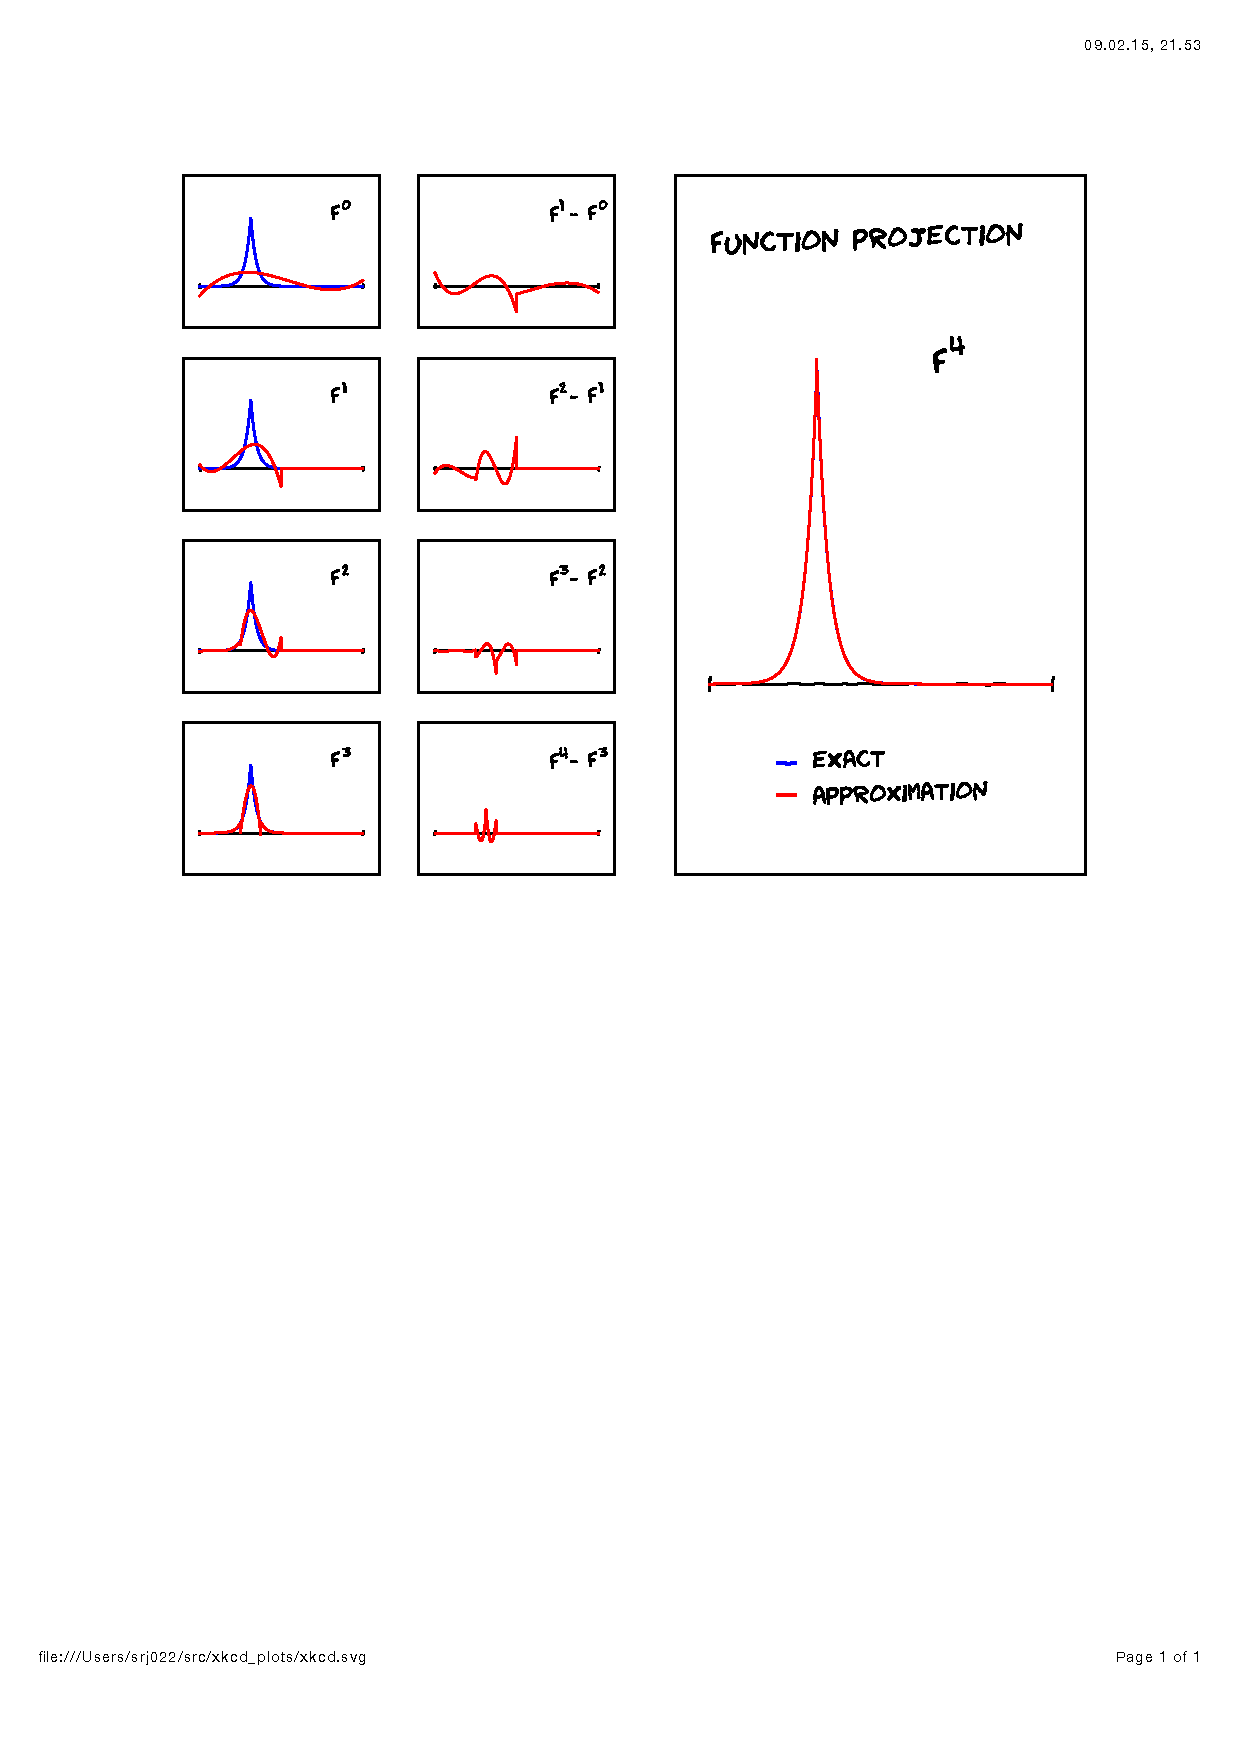
\includegraphics[scale=1.3, viewport = 85 420 550 760, clip]{figures/func_rep_2.pdf}
    \footnotesize
    \centering
    \\\textbf{Figure 1}: Scaling and wavelet projections of an s-type orbital.
\end{textblock} 

\begin{textblock}{7.0}(10.0,4.0)
    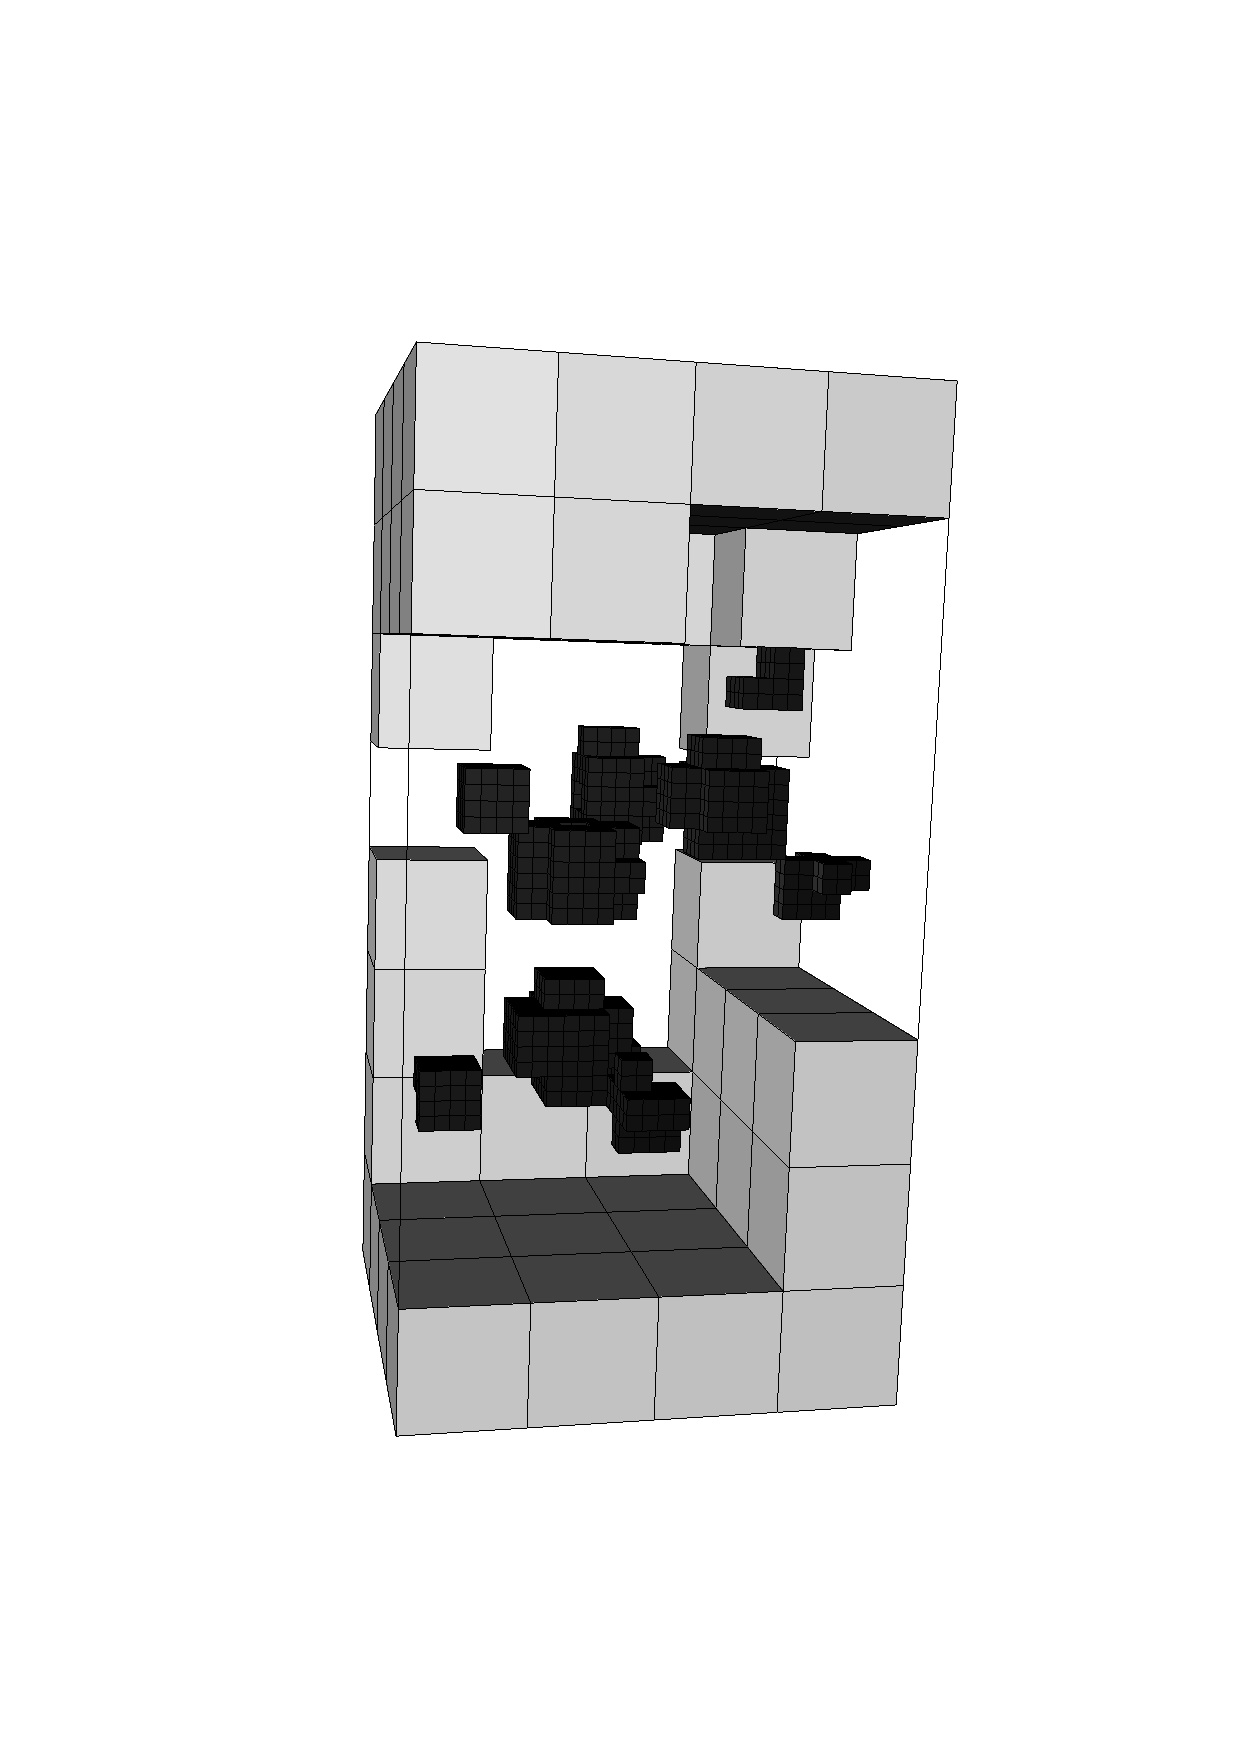
\includegraphics[angle=-90, scale=1.40, viewport = 170 150 470 700, clip]{figures/grid.pdf}
    \footnotesize
    \centering
    \\\textbf{Figure 2}: Adaptive grid for electron density of methyloxirane.
\end{textblock} 

\begin{textblock}{3.0}(14.2,9.0)
    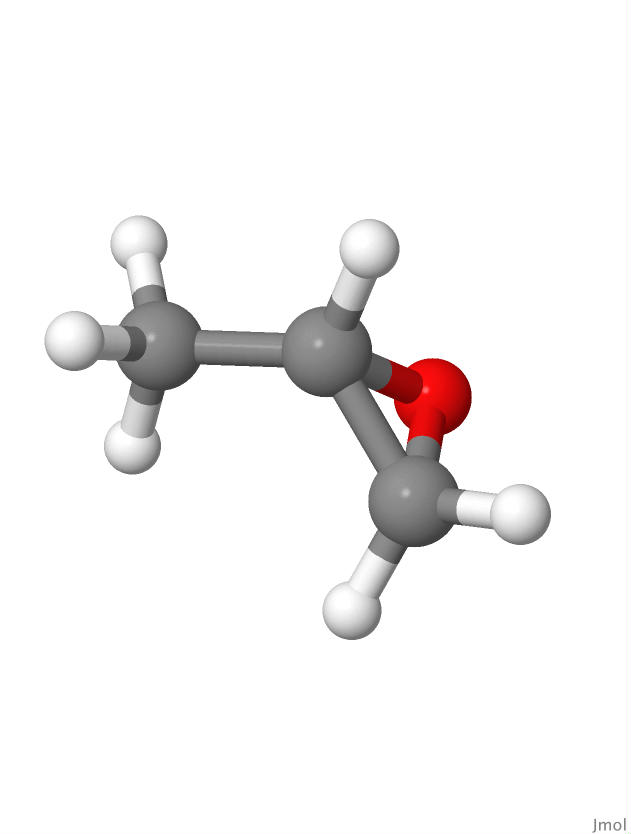
\includegraphics[scale=0.60, viewport = 0 180 550 650, clip]{figures/methyloxirane_white.jpg}
    \footnotesize
    \centering
    \\\textbf{Figure 3}: Methyloxirane molecule.
\end{textblock} 

\begin{textblock}{7}(10,8.1)
\footnotesize
\textbf{Table 1}: Total energies at Hartree-Fock and LDA (SVWN5) levels of theory. GTO
calculations by Dalton\cite{Dalton}. In the MRChem calculations, the orbitals are converged 
to the given threshold (the overall accuracy in the calculations is set two orders of magnitude
higher in order to get quadratic convergence in the energy).  
\begin{table}
    \normalsize
    \centering
    \begin{tabular}{|r|cc|cc|}
\hline                   &\multicolumn{2}{c|}{\textbf{Energy (a.u.)}}
						 &\multicolumn{2}{c|}{\textbf{CH$_3$CHCH$_2$O}}\\

                         &Hartree-Fock   &LDA        &               &               \\
\hline  \hspace{55mm}\   &\hspace{62mm}\ &\hspace{62mm}\ &\hspace{62mm}\ &\hspace{62mm}\ \\
	MRChem $10^{-2}$ & -192.0425     & -191.5975     &               &               \\
	MRChem $10^{-3}$ & -192.0002     & -191.5622     &               &               \\
	MRChem $10^{-4}$ & -192.0000     & -191.5619     &               &               \\
	                 &               &               &               &               \\
    aug-cc-pVQZ      & -191.9968     & -191.5563     &               &               \\
%	aug-cc-pVTZ      & -191.9850     & -191.5432     &               &               \\
	aug-cc-pVDZ      & -191.9357     & -191.4817     &               &               \\
	    cc-pVQZ      & -191.9960     & -191.5549     &               &               \\
%	    cc-pVTZ      & -191.9823     & -191.5396     &               &               \\
	    cc-pVDZ      & -191.9232     & -191.4622     &               &               \\
	                 &               &               &               &               \\
\hline
	\end{tabular}
    \end{table}
\end{textblock}

\begin{textblock}{7}(10,11.8)
\footnotesize
\textbf{Table 2}: Polarizability and optical rotation calculated at LDA (SVWN5) 
level of theory. Dynamic response at the sodium D line (589.3 nm) wavelength.
GTO calculations using gauge-including atomic orbitals (GIAO) by Dalton\cite{Dalton}.
\begin{table}
    \normalsize
    \centering
    \begin{tabular}{|r|cc|rr|}
	\hline&
        \multicolumn{2}{c|}{\textbf{Polarizability (a.u.)}}&
        \multicolumn{2}{c|}{\textbf{Optical rotation (a.u.)}}\\
                         & Static        & Dynamic       &
                         \multicolumn{1}{c}{$\beta$}&
                         \multicolumn{1}{c|}{$\alpha$}\\
	\hline
	\hspace{55mm}\   &\hspace{62mm}\ &\hspace{62mm}\ &\hspace{62mm}\ &\hspace{62mm}\ \\
%LDA
	MRChem $10^{-2}$ & 44.0764       & 45.2747       & 0.009376\ \ \ \ \ \ \ &   6.2440\ \ \ \ \ \ \ \ \ \\
	MRChem $10^{-3}$ & 44.0939       & 45.2907       & 0.010427\ \ \ \ \ \ \ &   6.9439\ \ \ \ \ \ \ \ \ \\
	MRChem $10^{-4}$ & 44.0935       & 45.2903       & 0.010556\ \ \ \ \ \ \ &   7.0298\ \ \ \ \ \ \ \ \ \\
	                 &               &               &                       &                           \\
	aug-cc-pVQZ      & 44.1326       & 45.3380       & 0.009861\ \ \ \ \ \ \ &   6.5669\ \ \ \ \ \ \ \ \ \\
%	aug-cc-pVTZ      & 44.1155       & 45.3170       & 0.009111\ \ \ \ \ \ \ &   6.0673\ \ \ \ \ \ \ \ \ \\
	aug-cc-pVDZ      & 44.0050       & 45.2025       & 0.000776\ \ \ \ \ \ \ &   0.5170\ \ \ \ \ \ \ \ \ \\
	    cc-pVQZ      & 42.3602       & 43.4064       & 0.001239\ \ \ \ \ \ \ &   0.8249\ \ \ \ \ \ \ \ \ \\
%	    cc-pVTZ      & 40.6143       & 41.5743       &-0.019612\ \ \ \ \ \ \ & -13.0606\ \ \ \ \ \ \ \ \ \\
	    cc-pVDZ      & 36.5586       & 37.3993       &-0.065879\ \ \ \ \ \ \ & -43.8711\ \ \ \ \ \ \ \ \ \\
	                 &               &               &               &               \\
%HF
%	MRChem $10^{-2}$ &               &               &               &               \\
%	MRChem $10^{-3}$ &               &               &               &               \\
%	MRChem $10^{-4}$ &               &               &               &               \\
%	                 &               &               &               &               \\
%	aug-cc-pV5Z      &               &               &               &               \\
%	aug-cc-pVQZ      & 38.1348       &               &  0.001713     &               \\
%	aug-cc-pVTZ      & 38.1219       & 38.83814      & -0.005394     &  -3.592310    \\
%	aug-cc-pVDZ      & 38.0229       & 38.73315      & -0.013018     &  -8.669360    \\
%	    cc-pV5Z      &               &               &               &               \\
%	    cc-pVQZ      & 37.2049       & 37.87318      & -0.008516     &  -5.671399    \\
%	    cc-pVTZ      & 36.0474       & 36.67956      & -0.017417     & -11.598786    \\
%	    cc-pVDZ      & 33.0901       & 33.66233      & -0.041624     & -27.718967    \\
%	                 &               &               &               &               \\
	\hline
	\end{tabular}
    \end{table}
\end{textblock}

\begin{textblock}{7}(10,15.3)
\footnotesize
\textbf{Table 3}: Magnetic properties calculated at
Hartree-Fock level of theory. GTO calculations by Dalton\cite{Dalton} 
with gauge-including atomic orbitals (GIAO). Magnetizabilities are also computed 
without GIAOs using different origins to test the origin dependence.
\begin{table}
    \normalsize
    \centering
    \begin{tabular}{|r|crr|ccc|}
\hline                   &\multicolumn{3}{c|}{\textbf{Magnetizability (a.u.)}}
                         &\multicolumn{3}{c|}{\textbf{NMR shielding (ppm)}}\\
                         & GIAO          & $(0,0,0)$\ \  & $(5,5,5)$\ \  &$\xi^{dia}$   & $\xi^{para}$  &$\xi^{tot}$    \\
\hline  \hspace{55mm}\   &\hspace{40mm}\ &\hspace{40mm}\ &\hspace{40mm}\ &\hspace{40mm}\ &\hspace{40mm}\ &\hspace{40mm}\ \\
%LDA
%	MRChem $10^{-2}$ &               &  -9.3721      &  -9.5864      &  444.6586     & -158.1337     &  286.5249     \\
%	MRChem $10^{-3}$ &               &  -9.3711      &  -9.3755      &  444.5783     & -150.3096     &  294.2687     \\
%	MRChem $10^{-4}$ &               &  -9.3726      &  -9.3823      &  444.4993     & -149.3424     &  295.1569     \\
%	                 &               &               &               &               &               &               \\
%	aug-cc-pVQZ      &               &               &               &               &               &               \\
%	aug-cc-pVTZ      & -9.3731       & -12.1930      & -53.1311      &  445.1985     & -147.3737     &  297.8248     \\
%	aug-cc-pVDZ      & -9.4211       & -15.2248      &-100.5931      &  448.0285     & -142.2480     &  305.7805     \\
%	    cc-pVQZ      & -9.3425       & -10.6651      & -28.4375      &  445.0422     & -148.4732     &  296.5690     \\
%	    cc-pVTZ      & -9.3224       & -13.2000      & -64.1239      &  445.4161     & -149.7417     &  295.6744     \\
%	    cc-pVDZ      & -9.1789       & -18.4454      &-133.9755      &  448.7952     & -146.7033     &  302.0919     \\
%	                 &               &               &               &               &               &               \\
%HF
	MRChem $10^{-2}$ &               &  -9.5497\ \ \ &  -9.9222\ \ \ &  446.7869     &  -96.6166     &  350.1703     \\
	MRChem $10^{-3}$ &               &  -9.4730\ \ \ &  -9.4363\ \ \ &  447.3444     &  -91.7855     &  355.5589     \\
	MRChem $10^{-4}$ &               &  -9.4758\ \ \ &  -9.4795\ \ \ &  447.3089     &  -90.9386     &  356.3704     \\
	                 &               &               &               &               &               &               \\
	aug-cc-pVQZ      & -9.4736       & -10.5253\ \ \ & -26.0533\ \ \ &  447.7508     &  -90.6691     &  357.0817     \\
%	aug-cc-pVTZ      & -9.4822       & -12.4117\ \ \ & -54.9201\ \ \ &  448.7949     &  -91.6336     &  357.1613     \\
	aug-cc-pVDZ      & -9.5369       & -15.4438\ \ \ &-101.6430\ \ \ &  451.0119     &  -88.5778     &  362.4341     \\
	    cc-pVQZ      & -9.4681       & -10.8019\ \ \ & -29.2395\ \ \ &  447.7833     &  -89.6304     &  358.1529     \\
%	    cc-pVTZ      & -9.4709       & -13.3872\ \ \ & -65.8671\ \ \ &  448.9517     &  -91.6778     &  357.2739     \\
	    cc-pVDZ      & -9.4924       & -19.0342\ \ \ &-140.0203\ \ \ &  451.6103     &  -87.4153     &  364.1950     \\
	                 &               &               &               &               &               &               \\
	\hline
	\end{tabular}
    \end{table}
\end{textblock}

\end{document}
